\chapter{AI: Agents}\label{AI: Agents}

\begin{figure}[H]
    \centering
    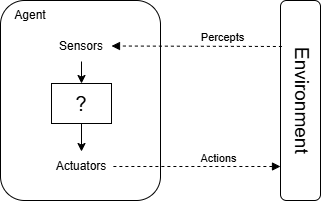
\includegraphics[
        width=0.5\linewidth, 
        height=4cm, 
        keepaspectratio
    ]{images/artificial-intelligence/ai-agents/agent-skeleton.drawio.png}
    \caption*{Agents interact with environments through sensors and actuators. \cite{common/online/tools/draw.io}}
\end{figure}


\begin{enumerate}[itemsep=0.2cm]
    \item \textbf{Agent}: An agent is anything that can be viewed as perceiving its environment through sensors and acting upon that environment through actuators.
    \hfill \cite{ai/book/Artificial-Intelligence-A-Modern-Approach/Russell-Norvig}

    \item \textbf{Environment}: environment refers to everything outside the agent that it interacts with.
    \hfill \cite{common/online/chatgpt}
    \\
    The “geography” of the environment is known \textbf{a priori}.
    \hfill \cite{ai/book/Artificial-Intelligence-A-Modern-Approach/Russell-Norvig}
    \\
    "A priori" : Knowledge or assumptions made before data is observed (e.g., predefined rules, constraints).
    \hfill \cite{common/online/chatgpt}

    \item \textbf{Sensors}: A sensor is any mechanism that allows an AI agent to perceive its environment by gathering information. This can be physical (hardware) or virtual (software).
    \hfill \cite{common/online/chatgpt}

    \item \textbf{Actuators}: An actuator is any mechanism that allows an AI agent to affect or change its environment by performing actions.
    \hfill \cite{common/online/chatgpt}

    \item \textbf{Percept}: agent’s perceptual inputs at any given instant
    \hfill \cite{ai/book/Artificial-Intelligence-A-Modern-Approach/Russell-Norvig}
    
    \item \textbf{Percept Sequence}: it is the complete history of everything the agent has ever perceived. In general, an agent’s choice of action at any given instant can depend on the entire percept sequence observed to date, but \textbf{not} on anything it hasn’t perceived.
    \hfill \cite{ai/book/Artificial-Intelligence-A-Modern-Approach/Russell-Norvig}

    \item \textbf{Agent Function}: maps any given percept sequence to an action; describes agent’s behavior; an external characterization of the agent; The agent function is an abstract mathematical description
    \hfill \cite{ai/book/Artificial-Intelligence-A-Modern-Approach/Russell-Norvig}

    \item \textbf{Agent Program}: internal implementation of the agent function for an artificial agent; the agent program is a concrete implementation, running within some physical system.
    \hfill \cite{ai/book/Artificial-Intelligence-A-Modern-Approach/Russell-Norvig}

    \item \textbf{Performance Measure}: It evaluates any given sequence of environment states.
    \hfill \cite{ai/book/Artificial-Intelligence-A-Modern-Approach/Russell-Norvig}

    \item \textbf{Rational Agent}: A rational agent is one that does the right thing
    \hfill \cite{ai/book/Artificial-Intelligence-A-Modern-Approach/Russell-Norvig}
    \\
    For each possible percept sequence, a rational agent should select an action that is expected to maximize its performance measure, given the evidence provided by the percept sequence and whatever built-in knowledge the agent has.
    \hfill \cite{ai/book/Artificial-Intelligence-A-Modern-Approach/Russell-Norvig}
    \\
    Rationality is not the same as perfection.
    \hfill \cite{ai/book/Artificial-Intelligence-A-Modern-Approach/Russell-Norvig}
    \\
    Rationality maximizes \textbf{expected} performance, while perfection maximizes \textbf{actual} performance.
    \hfill \cite{ai/book/Artificial-Intelligence-A-Modern-Approach/Russell-Norvig}
    \\
    Our definition of rationality does not require omniscience, then, because the rational choice depends only on the percept sequence to date
    \hfill \cite{ai/book/Artificial-Intelligence-A-Modern-Approach/Russell-Norvig}


    \item \textbf{Omniscient Agent}: An omniscient agent knows the actual outcome of its actions and can act accordingly; but omniscience is impossible in reality. 
    \hfill \cite{ai/book/Artificial-Intelligence-A-Modern-Approach/Russell-Norvig}


    \item \textbf{Information Gathering}: It is doing actions in order to modify future percepts.
    \hfill \cite{ai/book/Artificial-Intelligence-A-Modern-Approach/Russell-Norvig}


    

    \item When an agent is plunked down in an environment, it generates a sequence of actions according to the percepts it receives. This sequence of actions causes the environment to go through a sequence of states. If the sequence is desirable, then the agent has performed well.
    \hfill \cite{ai/book/Artificial-Intelligence-A-Modern-Approach/Russell-Norvig}

    \item  If we define success in terms of agent’s opinion of its own performance, an agent could achieve perfect rationality simply by deluding itself that its performance was perfect. 
    \hfill \cite{ai/book/Artificial-Intelligence-A-Modern-Approach/Russell-Norvig}

    \item Human agents in particular are notorious for “sour grapes” - believing they did not really want something (e.g., a Nobel Prize) after not getting it.
    \hfill \cite{ai/book/Artificial-Intelligence-A-Modern-Approach/Russell-Norvig}

    \item As a general rule, it is better to design performance measures according to what one actually wants in the environment, rather than according to how one thinks the agent should behave.
    \hfill \cite{ai/book/Artificial-Intelligence-A-Modern-Approach/Russell-Norvig}

    \item The agent’s initial configuration could reflect some prior knowledge of the environment, but as the agent gains experience this may be modified and augmented. There are extreme cases in which the environment is completely known \textbf{a priori}. In such cases, the agent need not perceive or learn; it simply acts correctly. Such agents are fragile.
    \hfill \cite{ai/book/Artificial-Intelligence-A-Modern-Approach/Russell-Norvig}

    \item To the extent that an agent relies on the prior knowledge of its designer rather than on its own percepts, we say that the agent \textbf{lacks autonomy}.
    \hfill \cite{ai/book/Artificial-Intelligence-A-Modern-Approach/Russell-Norvig}
    \\
    A rational agent should be \textbf{autonomous} - it should learn what it can to compensate for partial or incorrect prior knowledge. 
    \hfill \cite{ai/book/Artificial-Intelligence-A-Modern-Approach/Russell-Norvig}

    \item After sufficient experience of its environment, the behavior of a rational agent can become effectively \textbf{independent} of its prior knowledge. Hence, the incorporation of learning allows one to design a single rational agent that will succeed in a vast variety of environments.
    \hfill \cite{ai/book/Artificial-Intelligence-A-Modern-Approach/Russell-Norvig}

    
\end{enumerate}




\section{Task Environment/ Problem \cite{ai/book/Artificial-Intelligence-A-Modern-Approach/Russell-Norvig}}


\begin{enumerate}[itemsep=0.2cm]
    \item Task environments are essentially the “problems” to which rational agents are the “solutions.”
    \hfill \cite{ai/book/Artificial-Intelligence-A-Modern-Approach/Russell-Norvig}

    
\end{enumerate}

\subsection{PEAS: Defining Problem}

\begin{enumerate}[itemsep=0.2cm]
    \item \textbf{Performance}: 
    \begin{enumerate}[itemsep=0.1cm]
        \item Desirable qualities
        \hfill \cite{ai/book/Artificial-Intelligence-A-Modern-Approach/Russell-Norvig}

        \item Defines how the success of the agent is evaluated.
        \hfill \cite{common/online/chatgpt}

        \item[] \textbf{Example}: In a self-driving car, performance can be measured by safety, fuel efficiency, and reaching the destination on time.
        \hfill \cite{common/online/chatgpt}
    \end{enumerate}

    \item \textbf{Environment}: 
    \begin{enumerate}[itemsep=0.1cm]
        \item The surroundings in which the agent operates.
        \hfill \cite{common/online/chatgpt}

        \item[] \textbf{Example}: For a self-driving car, the environment includes roads, traffic, pedestrians, and weather conditions.
        \hfill \cite{common/online/chatgpt}
    \end{enumerate}

    \item \textbf{Actuators}: 
    \begin{enumerate}[itemsep=0.1cm]
        \item The mechanisms that allow the agent to take action.
        \hfill \cite{common/online/chatgpt}

        \hfill Can be hardware or software.

        \item[] \textbf{Example}: A self-driving car uses its steering wheel, accelerator, and brakes as actuators.
        \hfill \cite{common/online/chatgpt}
    \end{enumerate}

    \item \textbf{Sensors}: 
    \begin{enumerate}[itemsep=0.1cm]
        \item The components that allow the agent to perceive its environment.
        \hfill \cite{common/online/chatgpt}

        \hfill Can be hardware or software.

        \item[] \textbf{Example}: A self-driving car has cameras, LiDAR, GPS, and speed sensors.
        \hfill \cite{common/online/chatgpt}
    \end{enumerate}

\end{enumerate}


\vspace{0.3cm}

\textbf{Note}:
\begin{enumerate}
    \item some \textbf{software agents} (or \textbf{software robots} or \textbf{softbots}) exist in rich, unlimited domains. 
    \hfill \cite{ai/book/Artificial-Intelligence-A-Modern-Approach/Russell-Norvig}

    
\end{enumerate}


\subsection{Properties of Task Environments \cite{ai/book/Artificial-Intelligence-A-Modern-Approach/Russell-Norvig}}

\begin{enumerate}[itemsep=0.3cm]
    \item \textbf{Fully observable, partially observable, unobservable}:
    \hfill \cite{ai/book/Artificial-Intelligence-A-Modern-Approach/Russell-Norvig}
    \begin{enumerate}
        \item \textbf{fully observable}: If an agent’s sensors give it access to the complete state of the environment at each point in time, then we say that the task environment is fully observable. 
        A task environment is effectively fully observable if the sensors detect all aspects that are \textbf{relevant} to the choice of action; relevance, in turn, depends on the performance measure.
        Fully observable environments are convenient because the agent need not maintain any internal state to keep track of the world. 
        \hfill \cite{ai/book/Artificial-Intelligence-A-Modern-Approach/Russell-Norvig}

        \vspace{0.2cm}

        \item \textbf{partially observable}: An environment might be partially observable because of noisy and inaccurate sensors or because parts of the state are simply missing from the sensor data.
        \hfill \cite{ai/book/Artificial-Intelligence-A-Modern-Approach/Russell-Norvig}

        \vspace{0.2cm}

        \item \textbf{unobservable}: If the agent has no sensors at all then the environment is unobservable. 
        The agent’s goals may still be achievable, sometimes with certainty.
        \hfill \cite{ai/book/Artificial-Intelligence-A-Modern-Approach/Russell-Norvig}
    \end{enumerate}

    \item \textbf{Single agent, multi-agent}: 
    \begin{enumerate}[itemsep=0.1cm]
        \item \textbf{Single agent}:  Only 1 agent is interacting in the given environment.

        \item \textbf{Multi-agent}: More than 1 agent (of same type or different types) interact in the given environment.
        \begin{enumerate}
            \item \textbf{Competitive Multi-agent}: Agents maximize their own performance at cost of other agents' performance.
            \\
            Examples: 2 agents playing Chess against each other; taxi-driving (competing for parking space)

            \item \textbf{Cooperative Multi-agent}: Agents take actions to maximize collective performance.
            \\
            Example: taxi-driving (avoiding collisions)

            \vspace{0.3cm}

            \item \textbf{communication} often emerges as a rational behavior in multiagent environments; in some competitive environments, \textbf{randomized behavior} is rational because it avoids the pitfalls of predictability.
            \hfill \cite{ai/book/Artificial-Intelligence-A-Modern-Approach/Russell-Norvig}
        \end{enumerate}
        
    \end{enumerate}


    \item \textbf{Deterministic, stochastic, uncertain}:
    \begin{enumerate}
        \item If the next state of the environment is completely determined by the current state and the action executed by the agent, then we say the environment is deterministic; otherwise, it is stochastic.
        \hfill \cite{ai/book/Artificial-Intelligence-A-Modern-Approach/Russell-Norvig}

        
    \end{enumerate}

\end{enumerate}












